\documentclass[tikz,border=5pt]{standalone}
\usepackage{amsmath,amssymb,txfonts}
\usetikzlibrary{arrows.meta,positioning,fit,calc}
\newcommand{\gcode}{G_{\mathrm{code}}}
\newcommand{\gstate}{G_{\mathrm{state}}}
\begin{document}
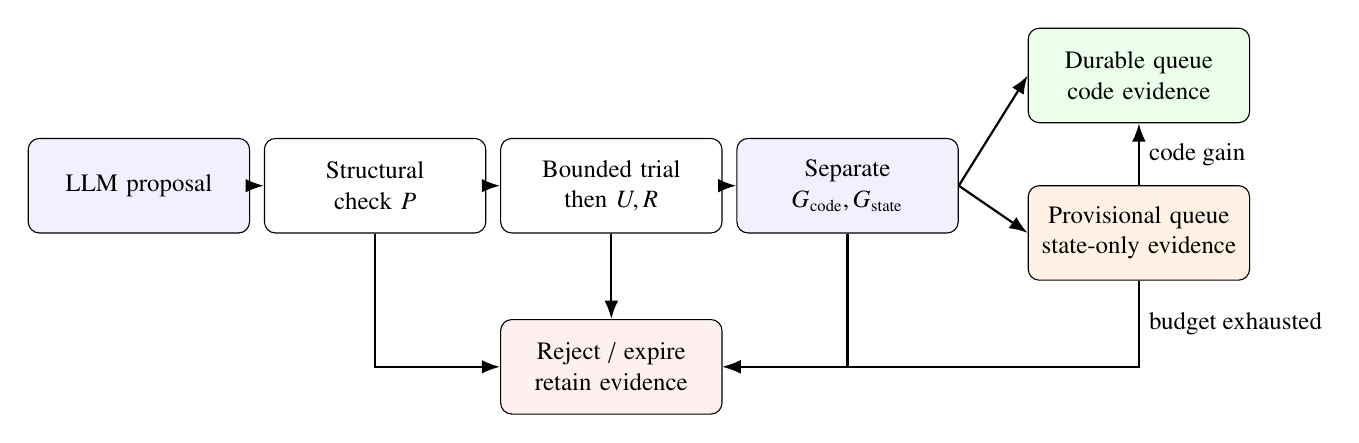
\begin{tikzpicture}[>=Latex,font=\small,
box/.style={draw,rounded corners,align=center,text width=26mm,minimum height=12mm,inner sep=3pt},
arr/.style={->,thick}]
\node[box,fill=blue!6] (llm) at (0,0) {LLM proposal};
\node[box] (p) at (3,0) {Structural\\check $P$};
\node[box] (trial) at (6,0) {Bounded trial\\then $U,R$};
\node[box,fill=blue!6] (gain) at (9,0) {Separate\\$\gcode,\gstate$};
\node[box,fill=green!8] (dur) at (12.7,1.4) {Durable queue\\code evidence};
\node[box,fill=orange!10] (prov) at (12.7,-.6) {Provisional queue\\state-only evidence};
\node[box,fill=red!6] (rej) at (6,-2.3) {Reject / expire\\retain evidence};
\draw[arr] (llm)--(p);
\draw[arr] (p)--(trial);
\draw[arr] (trial)--(gain);
\draw[arr] (gain.east)--(dur.west);
\draw[arr] (gain.east)--(prov.west);
\draw[arr] (p.south)|-(rej.west);
\draw[arr] (trial.south)--(rej.north);
\draw[arr] (gain.south)|-(rej.east);
\draw[arr] (prov.south)|-node[pos=.25,right]{budget exhausted}(rej.east);
\draw[arr] (prov.north)--node[right]{code gain}(dur.south);

\path (llm.south west);\pgfgetlastxy{\figx}{\figy}\typeout{FIG2|llm|sw|\figx|\figy}
\path (llm.north east);\pgfgetlastxy{\figx}{\figy}\typeout{FIG2|llm|ne|\figx|\figy}
\path (p.south west);\pgfgetlastxy{\figx}{\figy}\typeout{FIG2|p|sw|\figx|\figy}
\path (p.north east);\pgfgetlastxy{\figx}{\figy}\typeout{FIG2|p|ne|\figx|\figy}
\path (trial.south west);\pgfgetlastxy{\figx}{\figy}\typeout{FIG2|trial|sw|\figx|\figy}
\path (trial.north east);\pgfgetlastxy{\figx}{\figy}\typeout{FIG2|trial|ne|\figx|\figy}
\path (gain.south west);\pgfgetlastxy{\figx}{\figy}\typeout{FIG2|gain|sw|\figx|\figy}
\path (gain.north east);\pgfgetlastxy{\figx}{\figy}\typeout{FIG2|gain|ne|\figx|\figy}
\path (dur.south west);\pgfgetlastxy{\figx}{\figy}\typeout{FIG2|dur|sw|\figx|\figy}
\path (dur.north east);\pgfgetlastxy{\figx}{\figy}\typeout{FIG2|dur|ne|\figx|\figy}
\path (prov.south west);\pgfgetlastxy{\figx}{\figy}\typeout{FIG2|prov|sw|\figx|\figy}
\path (prov.north east);\pgfgetlastxy{\figx}{\figy}\typeout{FIG2|prov|ne|\figx|\figy}
\path (rej.south west);\pgfgetlastxy{\figx}{\figy}\typeout{FIG2|rej|sw|\figx|\figy}
\path (rej.north east);\pgfgetlastxy{\figx}{\figy}\typeout{FIG2|rej|ne|\figx|\figy}
\end{tikzpicture}
\end{document}
